%%%%%%%%%%%%%%%%%%%%%%%%%%%%%%%%%%%%%%%%%
% Beamer Presentation
% LaTeX Template
% Version 1.0 (10/11/12)
%
% This template has been downloaded from:
% http://www.LaTeXTemplates.com
%
% License:
% CC BY-NC-SA 3.0 (http://creativecommons.org/licenses/by-nc-sa/3.0/)
%
%%%%%%%%%%%%%%%%%%%%%%%%%%%%%%%%%%%%%%%%%

%----------------------------------------------------------------------------------------
%	PACKAGES AND THEMES
%----------------------------------------------------------------------------------------

\documentclass{beamer}

\mode<presentation> {

% The Beamer class comes with a number of default slide themes
% which change the colors and layouts of slides. Below this is a list
% of all the themes, uncomment each in turn to see what they look like.

%\usetheme{default}
%\usetheme{AnnArbor}
%\usetheme{Antibes}
%\usetheme{Bergen}
%\usetheme{Berkeley}
%\usetheme{Berlin}
%\usetheme{Boadilla}
%\usetheme{CambridgeUS}
%\usetheme{Copenhagen}
%\usetheme{Darmstadt}
%\usetheme{Dresden}
%\usetheme{Frankfurt}
%\usetheme{Goettingen}
%\usetheme{Hannover}
%\usetheme{Ilmenau}
%\usetheme{JuanLesPins}
%\usetheme{Luebeck}
\usetheme{Madrid}
%\usetheme{Malmoe}
%\usetheme{Marburg}
%\usetheme{Montpellier}
%\usetheme{PaloAlto}
%\usetheme{Pittsburgh}
%\usetheme{Rochester}
%\usetheme{Singapore}
%\usetheme{Szeged}
%\usetheme{Warsaw}

% As well as themes, the Beamer class has a number of color themes
% for any slide theme. Uncomment each of these in turn to see how it
% changes the colors of your current slide theme.

%\usecolortheme{albatross}
%\usecolortheme{beaver}
%\usecolortheme{beetle}
%\usecolortheme{crane}
%\usecolortheme{dolphin}
%\usecolortheme{dove}
%\usecolortheme{fly}
%\usecolortheme{lily}
%\usecolortheme{orchid}
%\usecolortheme{rose}
%\usecolortheme{seagull}
%\usecolortheme{seahorse}
%\usecolortheme{whale}
%\usecolortheme{wolverine}

%\setbeamertemplate{footline} % To remove the footer line in all slides uncomment this line
%\setbeamertemplate{footline}[page number] % To replace the footer line in all slides with a simple slide count uncomment this line

%\setbeamertemplate{navigation symbols}{} % To remove the navigation symbols from the bottom of all slides uncomment this line
}

\usepackage{graphicx} % Allows including images
\usepackage{booktabs} % Allows the use of \toprule, \midrule and \bottomrule in tables

%----------------------------------------------------------------------------------------
%	TITLE PAGE
%----------------------------------------------------------------------------------------

\title[Vowel Classification]{Training Support Vector Machines for SAE Vowel Phoneme Classification} % The short title appears at the bottom of every slide, the full title is only on the title page

\author{Alan J. Zaffetti} % Your name
\institute[UMASS Amherst] % Your institution as it will appear on the bottom of every slide, may be shorthand to save space
{
University of Massachusetts Amherst \\ % Your institution for the title page
\medskip
\textit{azaffett@umass.edu} % Your email address
}
\date{\today} % Date, can be changed to a custom date

\begin{document}

\begin{frame}
\titlepage % Print the title page as the first slide
\end{frame}

\begin{frame}
\frametitle{Overview} % Table of contents slide, comment this block out to remove it
\tableofcontents % Throughout your presentation, if you choose to use \section{} and \subsection{} commands, these will automatically be printed on this slide as an overview of your presentation
\end{frame}

%----------------------------------------------------------------------------------------
%	PRESENTATION SLIDES
%----------------------------------------------------------------------------------------

%------------------------------------------------
\section{Domain Overview} % Sections can be created in order to organize your presentation into discrete blocks, all sections and subsections are automatically printed in the table of contents as an overview of the talk
%------------------------------------------------

\begin{frame}
\frametitle{Vowel Phonemes}
\begin{itemize}
\item Phonemes are the units of sound in an utterance.
\item Vowel phonemes are found at nucleus of syllable.
\item \begin{tabular}{lll}
sh\textbf{i}p & b\textbf{oo}k & \textbf{e}gg \\
c\textbf{a}t & c\textbf{u}p & h\textbf{o}t 
\end{tabular}
\item Here are some more of them:
\begin{tabular}{llll}
ae="had" & ah="hod" & aw="hawed" & eh="head" \\
er="heard" & ei="haid" & ih="hid" & iy="heed" \\
oa="boat" & oo="hood" & uh="hud" & uw="who'd")
\end{tabular}
\end{itemize}
\end{frame}

%------------------------------------------------

\begin{frame}
\frametitle{Classifying Phonemes}
\begin{block}{Praat Spectrogram}
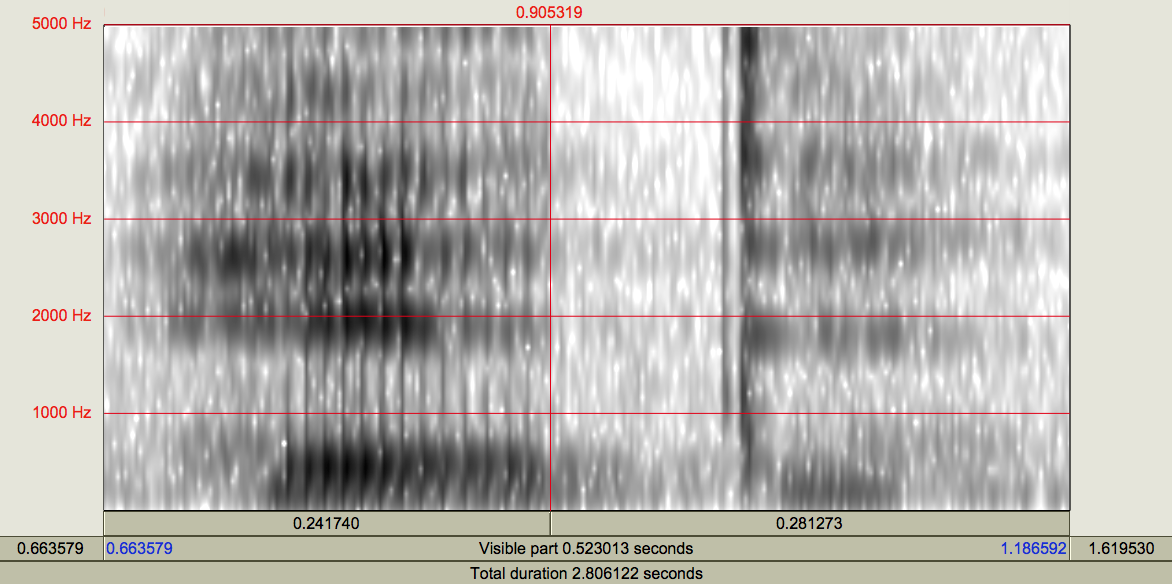
\includegraphics[scale=.28]{../figures/hid-spectrogram.png}
\end{block}
\end{frame}

%------------------------------------------------

\begin{frame}
\frametitle{Classifying Phonemes}
\begin{block}{Phoneme Classification}
"The task of deciding what the phonetic identity of a speech utterance is." \cite{p1}
\end{block}
\begin{itemize}
\item In speech recognition this means learning a model from data.
\item One such model is Support Vector Machines. 
\end{itemize}
\end{frame}

%------------------------------------------------

\section{Intro to Support Vector Machines}

%------------------------------------------------

\begin{frame}
\frametitle{Support Vector Machines (SVM)}
\begin{columns}[c] % The "c" option specifies centered vertical alignment while the "t" option is used for top vertical alignment

\column{.45\textwidth} % Left column and width

\begin{block}{SVM}
\begin{enumerate}
\item A binary linear classifier capable of learning from example.
\item Represents data as points in space and partitions them over a line (via MMP).
\end{enumerate}
\end{block}

\begin{itemize}
\item Linear equations partition space in $\Re^2$.
\item \textbf{+1} class and \textbf{-1} class.
\end{itemize}

\column{.5\textwidth} % Right column and width

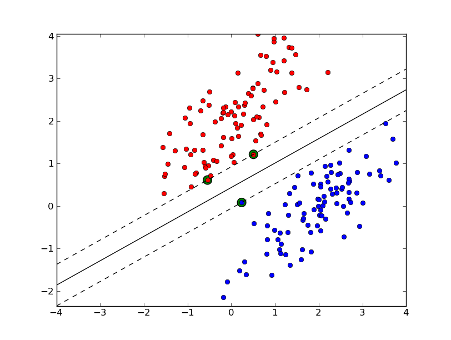
\includegraphics[scale=.5]{../figures/svm-linear.png}

\end{columns}
\end{frame}

%------------------------------------------------

\begin{frame}
\frametitle{MMDP and Support Vectors}
\begin{columns}[c]

\column{.45\textwidth}

\begin{block}{MMD Principle}
If the training data are linearly separable:
\begin{enumerate}
\item Select two lines in a way that they separate the data and there are no points between them.
\item Try to maximize their distance.
\end{enumerate}
This leads to lesser generalization error. Leaves room for new data, noise.
\end{block}

\column{.5\textwidth}

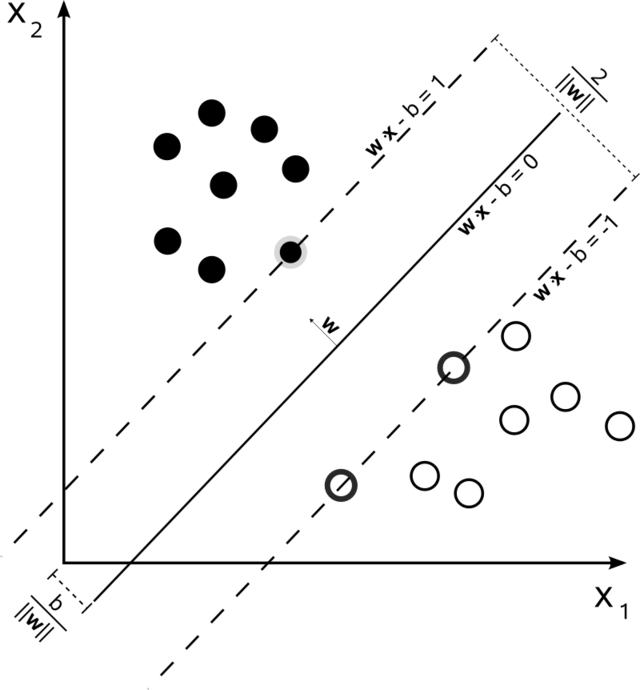
\includegraphics[scale=.2]{../figures/mm-hyperplane.png}

\end{columns}

\end{frame}

%------------------------------------------------

\begin{frame}
\frametitle{Linear Seperability}
\begin{columns}[c]

\column{.45\textwidth}

\begin{itemize}
\item The graph on the left represents data in $\Re^1$.
\end{itemize}

\begin{quote}
Are the two classes linearly seperable?
\end{quote}

\begin{quote}
Is it possible to draw a straight line?
\end{quote}

\column{.5\textwidth}

\begin{block}{Strange Data}
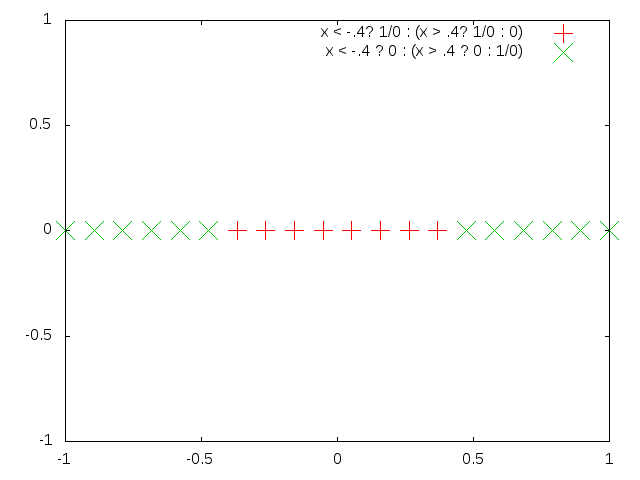
\includegraphics[scale=.35]{../figures/example_0.png}
\end{block}

\end{columns}

\end{frame}

%------------------------------------------------

\begin{frame}
\frametitle{Linear Seperability}
\begin{columns}[c]

\column{.45\textwidth}

\begin{itemize}
\item Yes! If you cheat.
\item Map each data point 
\begin{align}
x\longrightarrow (x,x^2)
\end{align}
\end{itemize}

\begin{theorem}[$\Re\rightarrow\Re^n$ Mapping]
This result generalizes:
\begin{align}
\forall D \exists n : \exists\ a\ linear\ cut\ in\ \Re^n
\end{align}
\end{theorem}


\column{.5\textwidth}

\begin{block}{Strange Data}
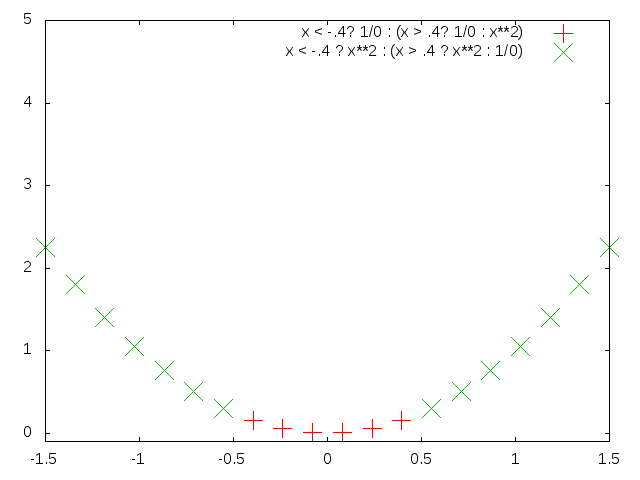
\includegraphics[scale=.35]{../figures/example_1.png}
\end{block}

\end{columns}

\end{frame}

%------------------------------------------------

\begin{frame}
\frametitle{Linear Seperability}

\begin{columns}[c]

\column{.54\textwidth}

\begin{columns}[c]

\column{.87\textwidth}
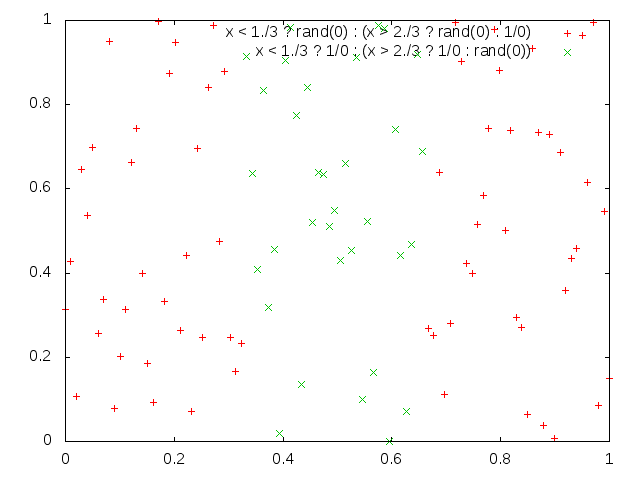
\includegraphics[scale=.31]{../figures/example_3.png}

\column{.1\textwidth} 
\begin{large}
$\longrightarrow$
\end{large}

\end{columns}

\column{.4\textwidth}

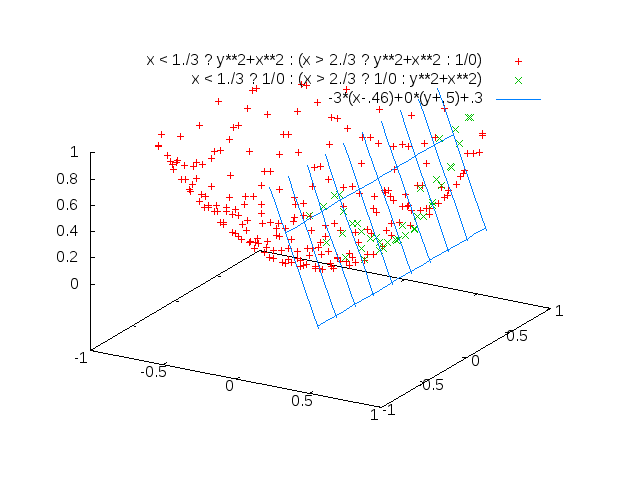
\includegraphics[scale=.31]{../figures/example_4.png}

\end{columns}

\end{frame}

%------------------------------------------------

\begin{frame}
\frametitle{Kernel Trick}

\begin{block}{Kernel Functions}
$\Phi$-mapping functions exist which map data to even higher dimensions, and don't share the same limitations as $\Re$-mapping.
\end{block}

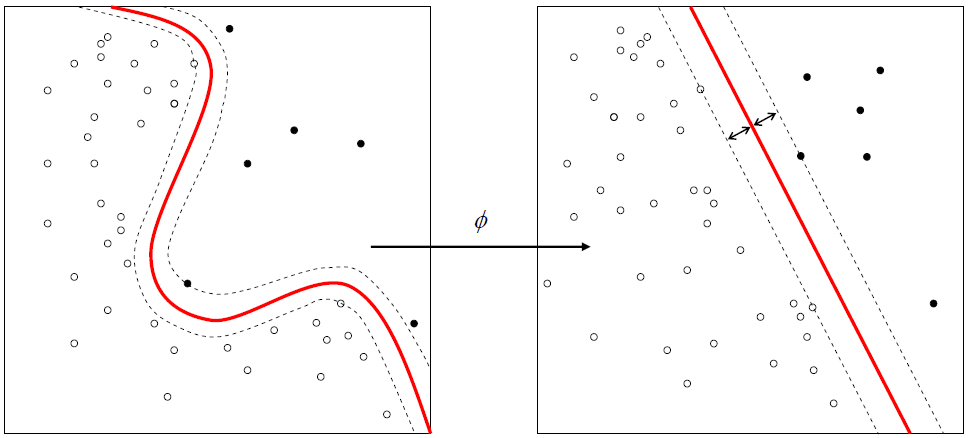
\includegraphics[scale=.45]{../figures/Kernel_Machine.png}

\end{frame}

%------------------------------------------------

\section{My Project}

%------------------------------------------------

\begin{frame}
\frametitle{Project Goals}

\begin{itemize}
\item Hillenbrand Vowel Formant dataset
\item Contains information on vowel length, formant frequency, speaker data.
\item Tune an SVM to recognize major vowel distinctions.
\end{itemize}

\begin{block}{SVM Feature Model}
Formally:
\begin{align}
(\Delta t,f0,\hat{f1},\hat{f2},\hat{f3},f4)\longrightarrow v\in V
\end{align}
Where $\Delta t$ is the length of the vowel, and $f_0\cdots f_4$ are formant data at different vowel durations, $v$ is a vowel class in $V$.
\end{block}

\end{frame}

%------------------------------------------------

\begin{frame}
\frametitle{Project Challenges}

\begin{block}{Challenge}
SVM are binary classifiers. They must be extended to work with multiple classes.
\end{block}

\begin{block}{Possible Solutions}
\begin{enumerate}
\item Create $O(n^2)$ classifiers for each vowel pair $(i\neq j)\implies (i,j)$ and chose the class which performs best on its $O(n)$ tests.
\item Create $O(n)$ cascading classifiers for each vowel $v$, testing $(v,\bar{v})$. Select the \textit{best} value.
\end{enumerate}

\end{block}

\begin{block}{Challenge}
Vowel classification is hard.
\end{block}

\end{frame}

%------------------------------------------------

\begin{frame}
\frametitle{Project Challenges}

\begin{columns}[c]

\column{.45\textwidth}

\begin{block}{Possible Solution}
SVMs accel at high-dimensional problems. More dimensionality could make the distinctions more clear, albeit more computationally intensive to decide. 
\end{block}

\column{.5\textwidth}

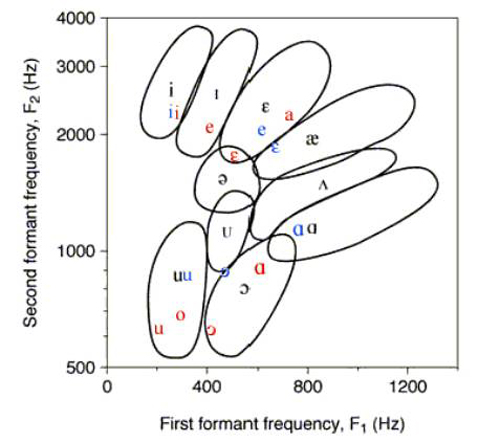
\includegraphics[scale=.45]{../figures/vowelchart.jpg}

\end{columns}

\end{frame}

%------------------------------------------------

\begin{frame}
\frametitle{References}
\footnotesize{
\begin{thebibliography}{99} % Beamer does not support BibTeX so references must be inserted manually as below
\bibitem[Boujelbene et. al., 2008]{p1} Boujelbene et. al. (2008)
\newblock Vowel Phoneme Classification Using SMO Algorithm for Training Support Vector 
Machines 
\newblock \emph{Information and Communication Technologies: From Theory to Applications} IEEE, 1 -- 5.
\end{thebibliography}
}
\end{frame}

%------------------------------------------------

\begin{frame}
\Huge{\centerline{The End}}
\end{frame}

%----------------------------------------------------------------------------------------

\end{document}